%Autores: Prof. Phyllipe Lima
%         Daylon Ramos da Silva
%Contato: phyllipe@inatel.br / phyllipe_slf@yahoo.com.br
%         biblioteca.pesquisa@inatel.br
%Modelo para escrita de artigos científicos para o TCC dos cursos Graduação do INATEL - Instituto Nacional de Telecomunicações. 
%Este template LaTeX é uma adaptação do modelo doc desenvolvido pelos professores Carlos Ynoguti e Dayan Guimarães

%Se você é novo no latex, um bom lugar para começar é
%https://pt.overleaf.com/learn
\documentclass[10pt,twocolumn]{article} 
%Use esse arquivo para incluir novos pacotes

\usepackage[%usado para determinar medidas
top=1.78cm,
bottom=1.78cm,
left=1.65cm,
right=1.65cm,
headsep=0cm,
%showframe
]{geometry}
%\usepackage[justification=centering]{caption}
\usepackage{inatel}%carregar algumas estilizacoes do inatel
\usepackage{times}
\usepackage{xcolor}
% initialize math tools
\usepackage{bm}
\usepackage{amsmath}
% sinc
\DeclareMathOperator{\sinc}{sinc}
\usepackage{cancel}
\usepackage{amssymb}
\usepackage{mathtools}
\usepackage{empheq}
\usepackage{arydshln}
\usepackage{steinmetz}
% define equal
\newcommand\eqdef{\mathrel{\overset{\makebox[0pt]{\mbox{\normalfont\tiny\sffamily def}}}{=}}}
% multirow in Tables
\usepackage{multirow}
% change title size
\usepackage{titlesec}
\titleformat*{\section}{\centering\huge}
% MATLAB Code Block
\usepackage[framed,numbered,autolinebreaks,useliterate]{mcode}
\usepackage{enumitem}%redefinir espacos itemize
\usepackage{graphicx}
\usepackage{url,hyperref}
\usepackage[utf8]{inputenc}
\usepackage{float}%mais controle para manipular figuras
\usepackage{caption}%manipular legenda da figura e tabela
\usepackage{mathtools}%equacoes
\usepackage[hang,flushmargin]{footmisc} 
\usepackage{xcolor}
\usepackage{wrapfig} %usado para envolver figura com texto
%\usepackage[portuguese]{babel}
\usepackage{fancyhdr}%criacao do cabecalho
\usepackage{etoolbox}
\usepackage{adjustbox}%mais controle para ajustar tamanho da tabela
\usepackage{comment}%ambiente para comentario
\usepackage{relsize} %usado por comandos \mathlarger
%\usepackage{mathptmx}

%Referencia bibliografica
\usepackage[
    style=numeric,
    sorting=none,
    maxbibnames=10]{biblatex}
\addbibresource{referencia.bib}

%Idioma. Use "english" para trabalhos em inglês
\usepackage[brazil]{babel}
%Ajustes na legenda da figura. Incluindo espacamento apos a legenda
\captionsetup[figure]{labelformat={default},labelsep=period,font=footnotesize, name=\footnotesize{Fig.},justification=raggedright,singlelinecheck=false,belowskip=-0.9\normalbaselineskip}
%\pagenumbering{gobble}

%Ajustes na legenda da tabela. 
\captionsetup[table]{labelformat={default},labelsep=newline,font={sc,footnotesize},justification=centering,singlelinecheck=false}

\renewcommand{\headrulewidth}{0pt}


\begin{document}

\title{\Huge \bf MTRN3020 Cheat Sheet}
\author{\large Currently maintained by: D.S.}

\maketitle

\section{Week 1}
\textbf{\large Final value theorem}
\begin{align*}
    \lim_{t\to \infty} &= \lim_{\color{red} s\to 0} \color{red} s \color{black} \cdot G(s) \\
    \lim_{t\to 0} &= \lim_{\color{red} s\to \infty} \color{red} s \color{black} \cdot G(s)
\end{align*}

\textbf{\large Block diagram simplifications}
\begin{figure}[H]
    \centering
    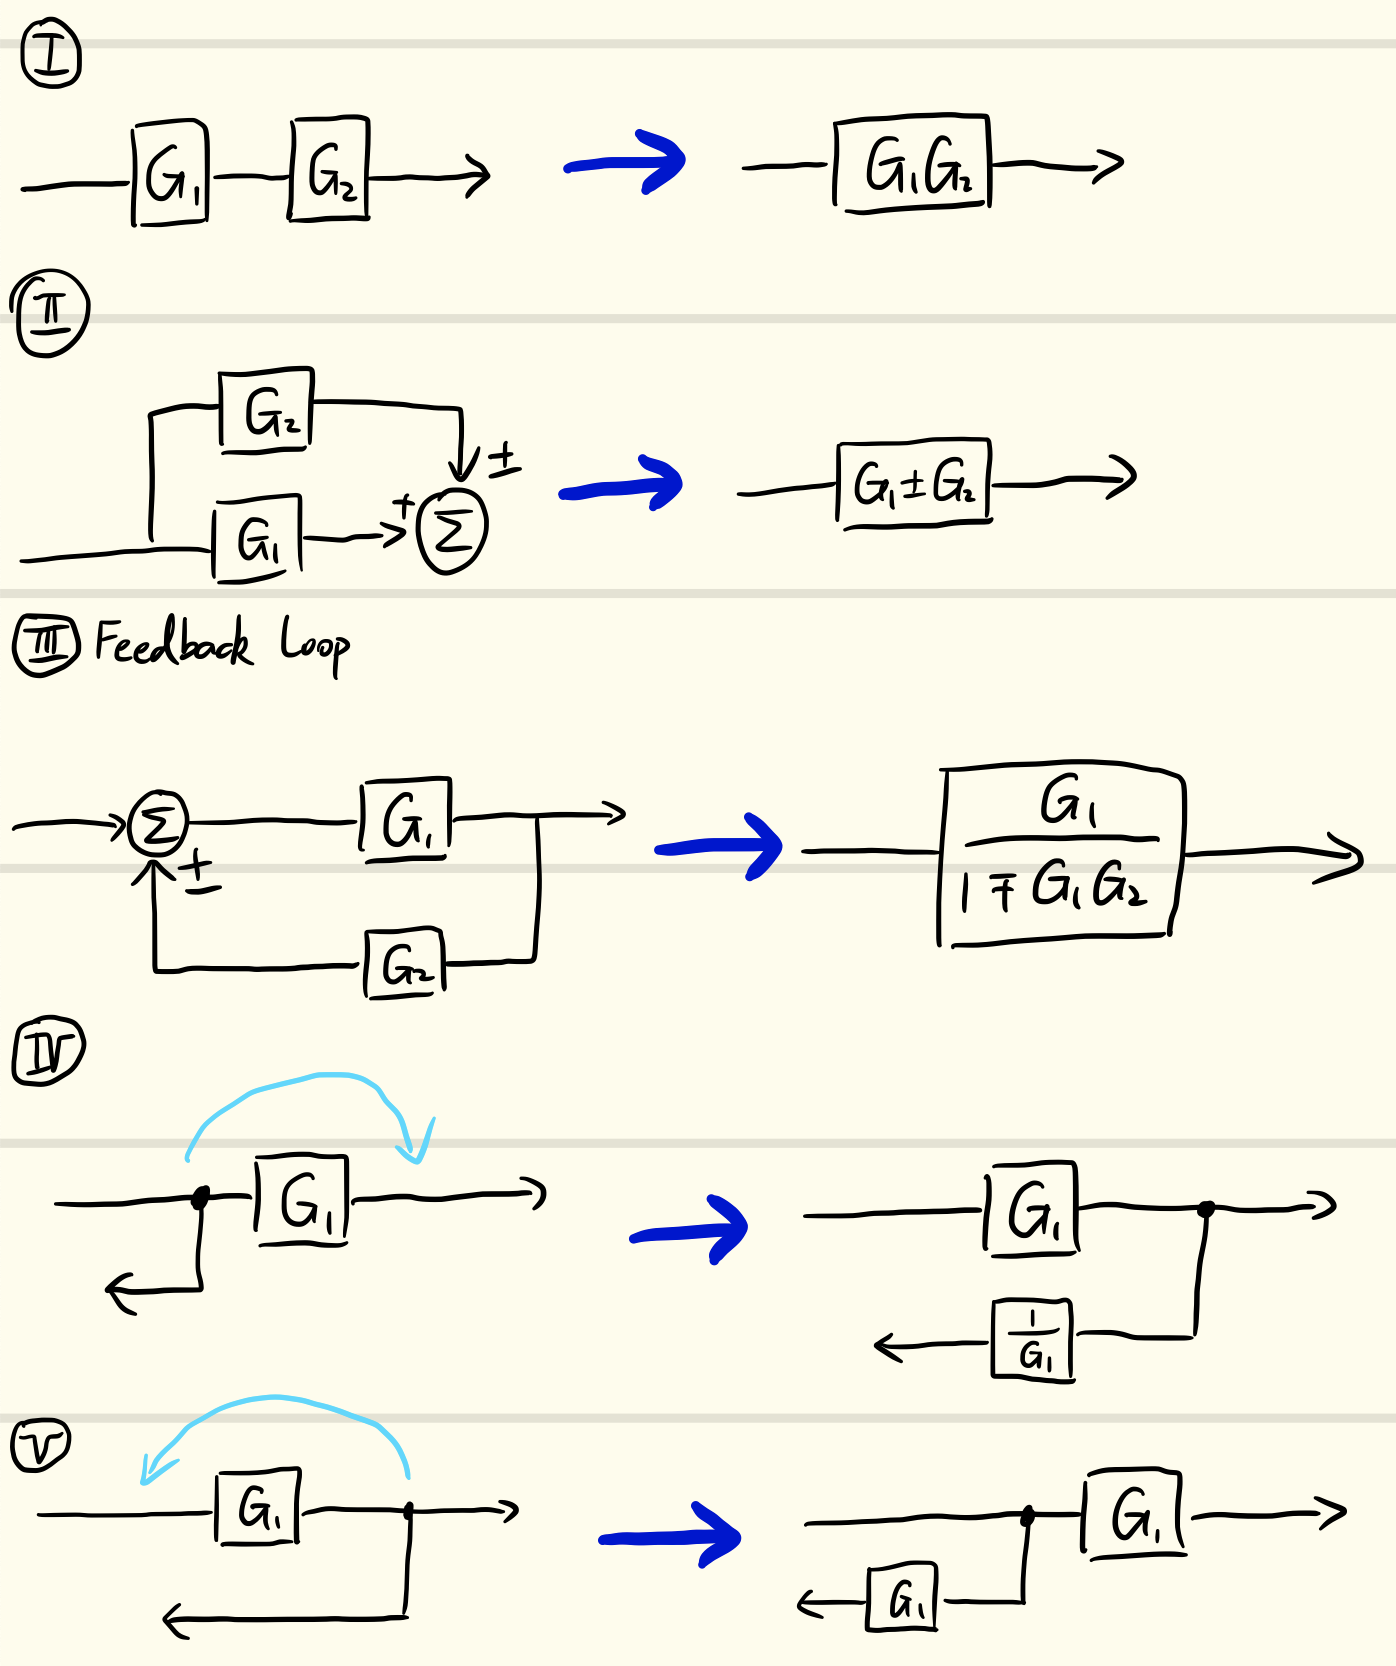
\includegraphics[width=0.25\textwidth]{images/block_diagram_simplification.png}
\end{figure}
\section{Week 2}
\textbf{\large Time Constants}
\begin{align*}
    \frac{1}{\tau s + 1} &\xrightarrow{\mathcal{L}^{-1}} e^{-\frac{1}{\tau} t} \to \; \text{smaller $\tau$, faster response} \\
    \frac{1}{s + a} &\xrightarrow{\mathcal{L}^{-1}} e^{-a t} \to \; \text{greater $a$, faster response}
\end{align*}

\textbf{\large Settling Time}
\begin{align*}
    t_s &= \frac{\ln(1-0.95)}{-a} \approx \frac{3}{\sigma} \\
    t_s &= \frac{\ln(1-0.98)}{-a} \approx \frac{4}{\sigma}
\end{align*}

\textbf{\large Second-order system damping ratio}
\begin{figure}[H]
    \centering
    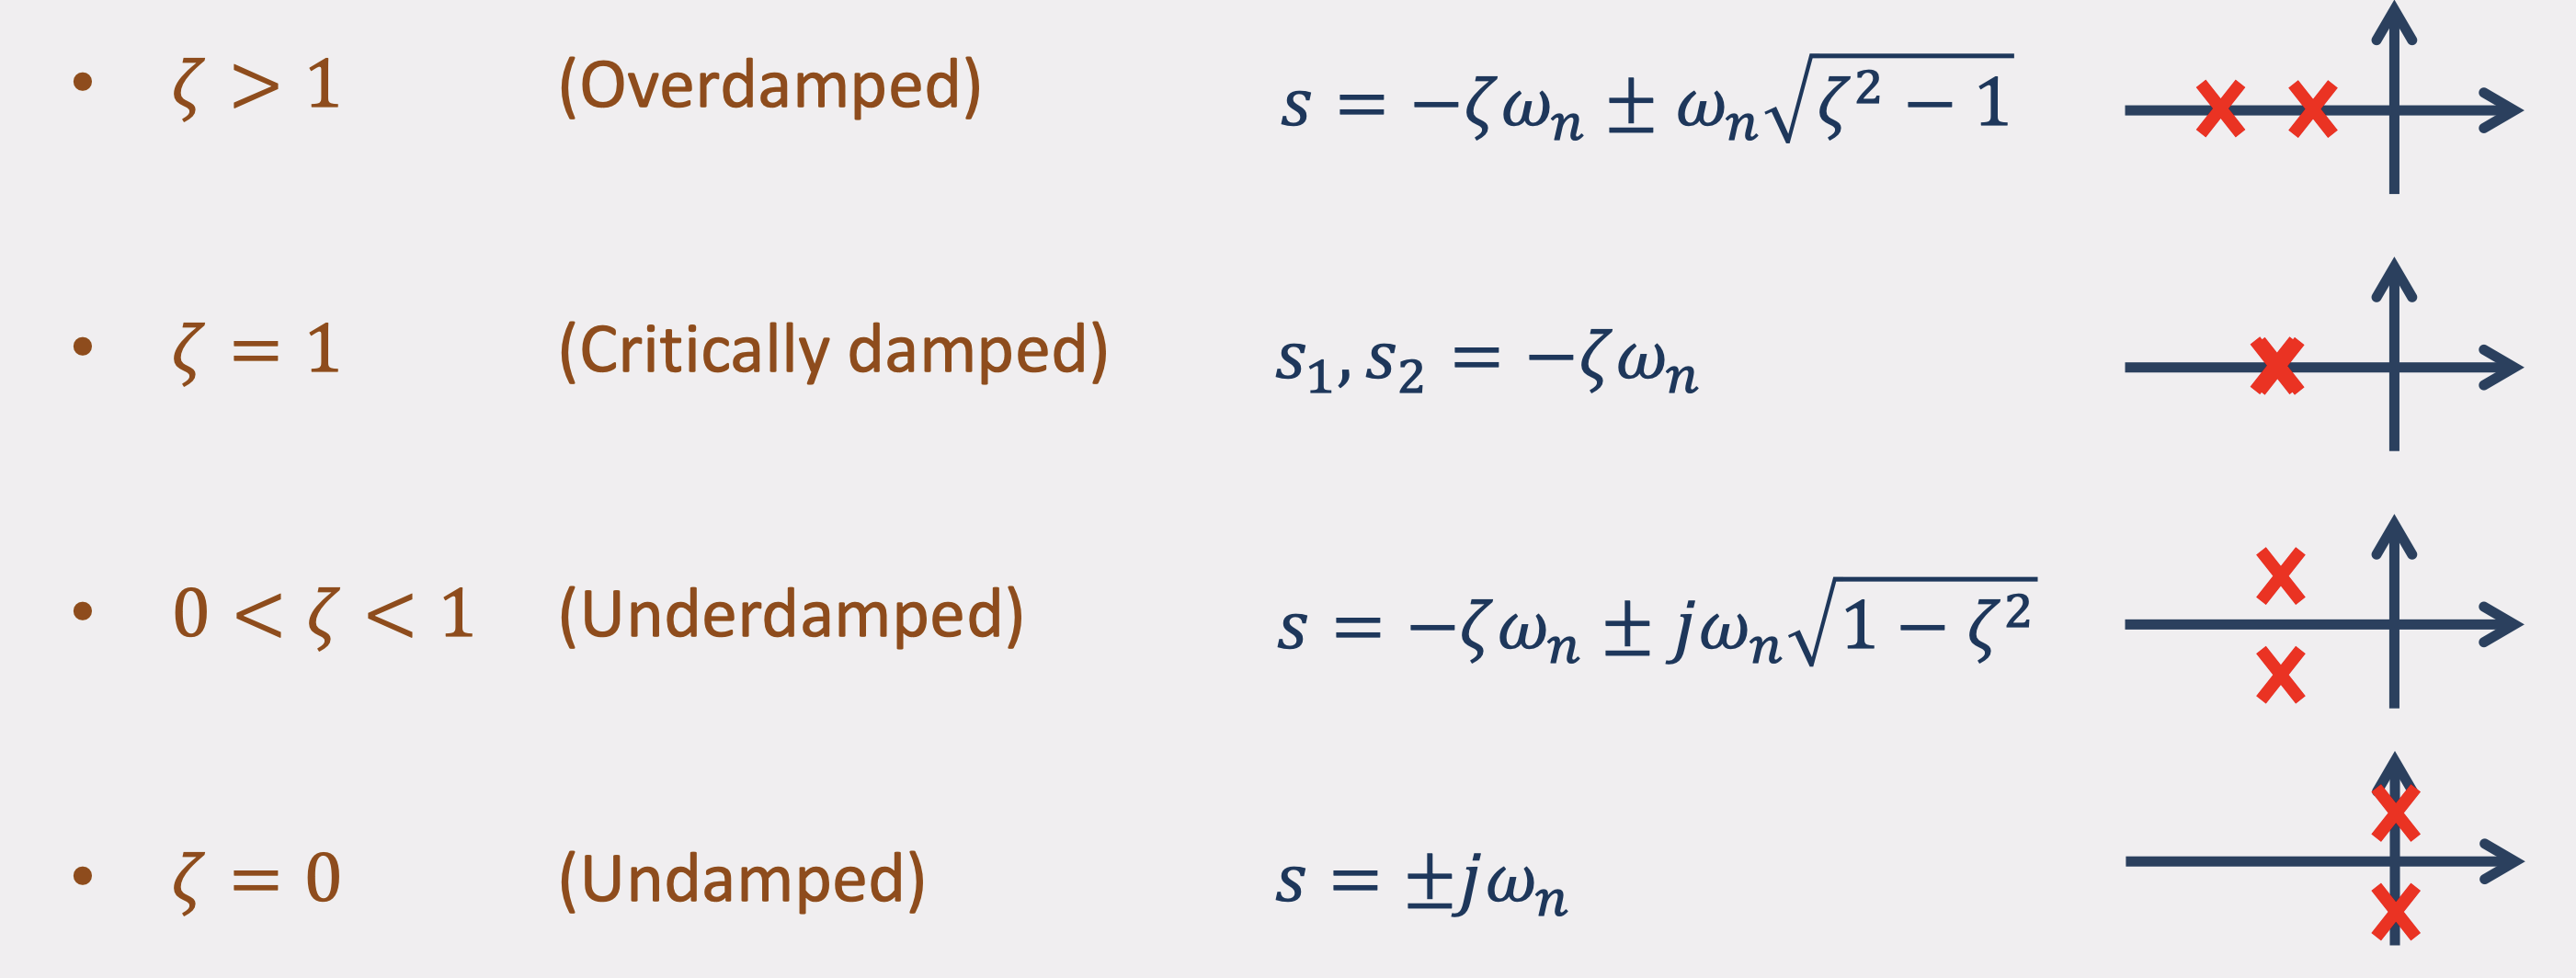
\includegraphics[width=0.45\textwidth]{images/damping_ratio.png}
\end{figure}
\vspace{1cm}

\textbf{\large S-plane parameters}
\begin{figure}[H]
    \centering
    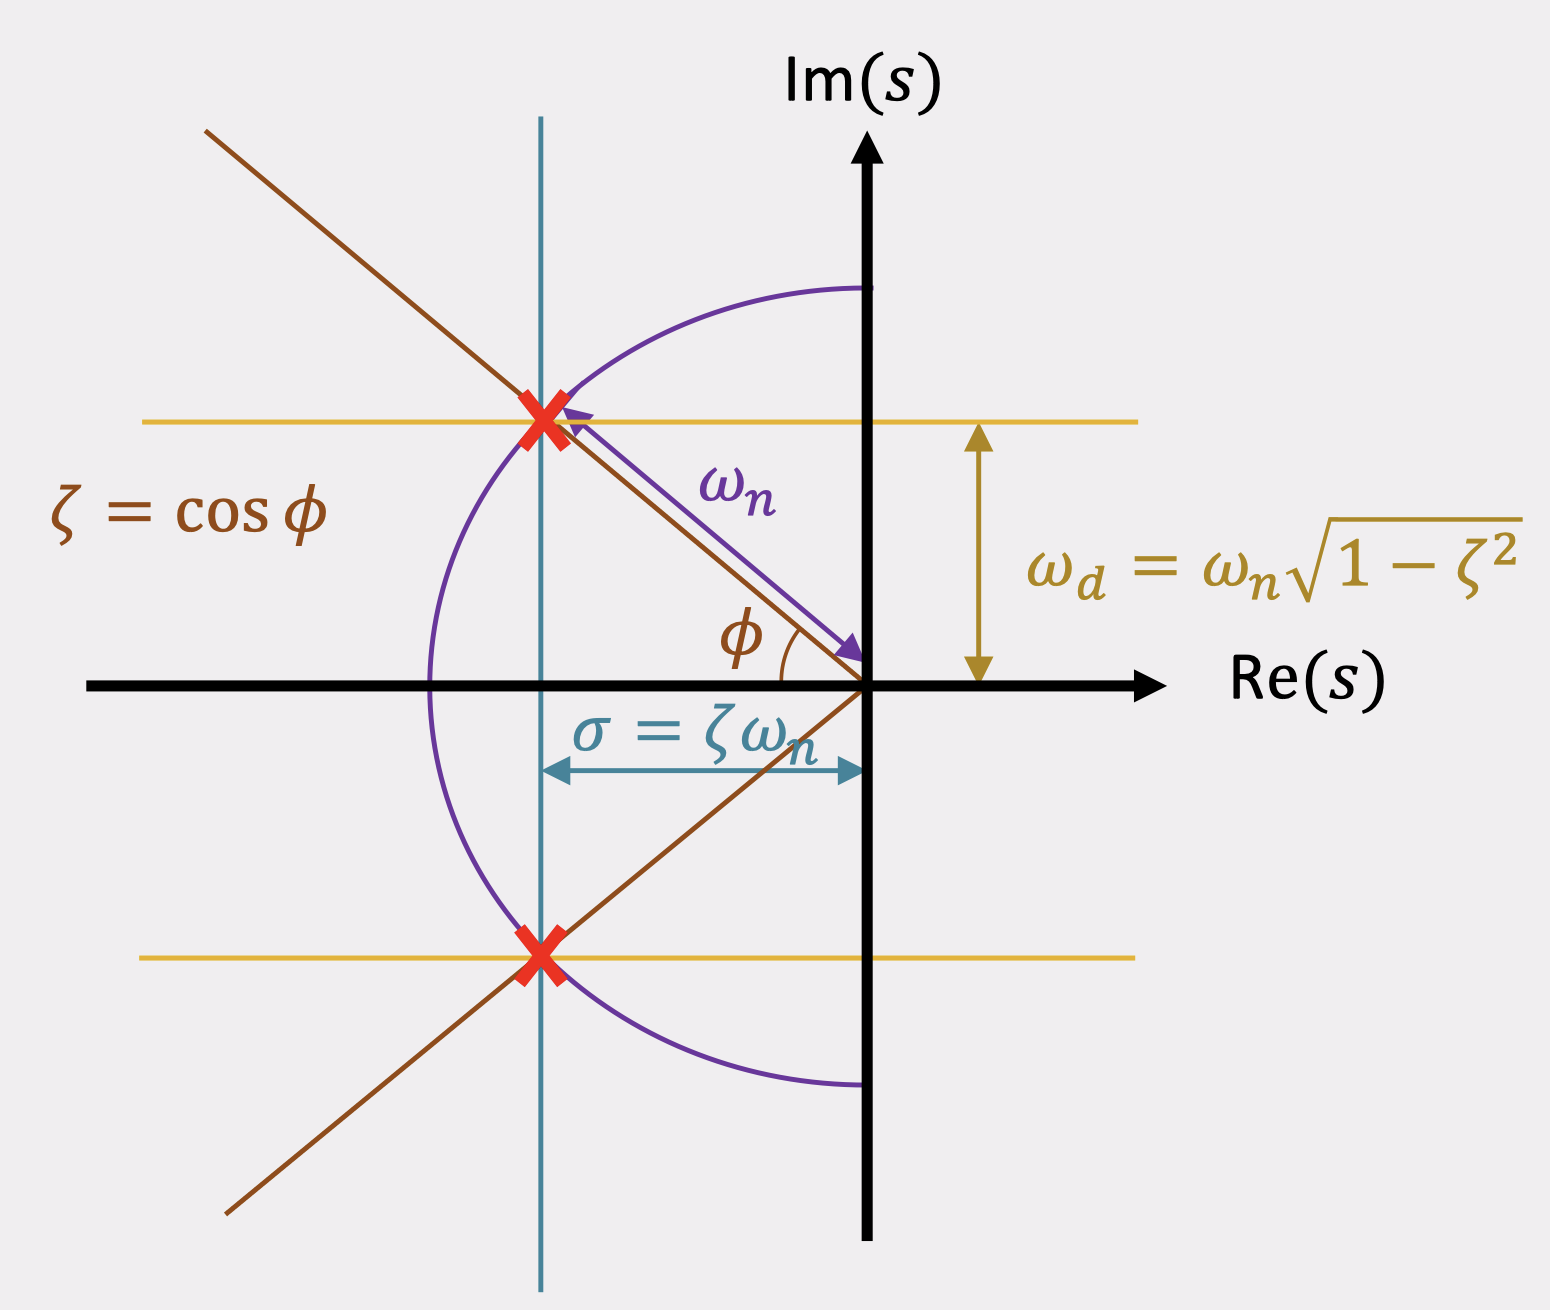
\includegraphics[width=0.45\textwidth]{images/s_plane_parameters.png}
\end{figure}

\textbf{\large Steady state gains}
\begin{itemize}
    \item \textbf{\underline{DC gain:}} 
    
    steady state of the unit step response.
    \begin{equation*}
        \text{DC Gain} = \lim_{s\to 0} G(s) 
    \end{equation*}
    \item \textbf{\underline{Instantaneous Gain:}} 
    
    initial value of the unit step response. 
    
    \textbf{All physical system should have zero Inst. Gain}.
    \begin{equation*}
        \text{Inst. Gain} = \lim_{s\to\infty} G(s)
    \end{equation*}
\end{itemize}


 

\textbf{\large Properness}
\begin{equation*}
    G(s) = \frac{s^n + a_{n-1}s^{n-1}+a_{n-2}s^{n-2}+\ldots + a_0}{s^m + b_{m-1}s^{m-1}+b_{m-2}s^{m-2}+\ldots + b_0}
\end{equation*}
\begin{itemize}
    \item \textbf{strictly proper when $m > n$ .} \\ Most physical/real system are strictly proper.
    \item \textbf{proper when $m = n$ .} \\ Discrete system (computer) is proper.
    \item \textbf{improper when $m < n$ .} \\ Cannot be physically implemented. Because in order to deliver a control signal \textbf{now}, you need to know a \textbf{future} input value.
\end{itemize}


\section{Week 3}
\textbf{Key concepts of Root Locus Plot}
\begin{itemize}
    \item RL plots the coordinates of closed loop poles, $s$, given different $K$ values using CE: $1+K\cdot G(s) = 0$.
    \item RL starts ($K=0$) at open-loop poles, and ends ($K\to \infty$) at either open-loop zeros or asymptotes. 
    \item Adding open-loop poles makes the closed-loop system \textbf{less stable}.
    \item Adding open-loop zeros makes the closed-loop system \textbf{more stable}. 
\end{itemize}

\textbf{Given s-value, how to find K-value?}
\begin{itemize}
    \item Magnitude Condition \\
    \begin{equation*}
        \frac{|s+a_0|\times |s+a_1| \times \ldots |s+a_m|}{|s+b_0|\times |s+b_1| \times \ldots |s+b_m|} = \left|-\frac{1}{K}\right|
    \end{equation*}
    \item Angle Condition ($\theta$ away from x-axis) \\
    \begin{equation*}
        \sum_{i=1}^{m} \phase{(s+a_i)} - \sum_{j=1}^{n}\phase{(s+b_j)} = \phase{-\frac{1}{K}} = -180^{\circ} \; (\text{if $K>0$})
    \end{equation*}
\end{itemize}

\textbf{Root Locus Drawing Rules}
\begin{figure}[H]
    \centering
    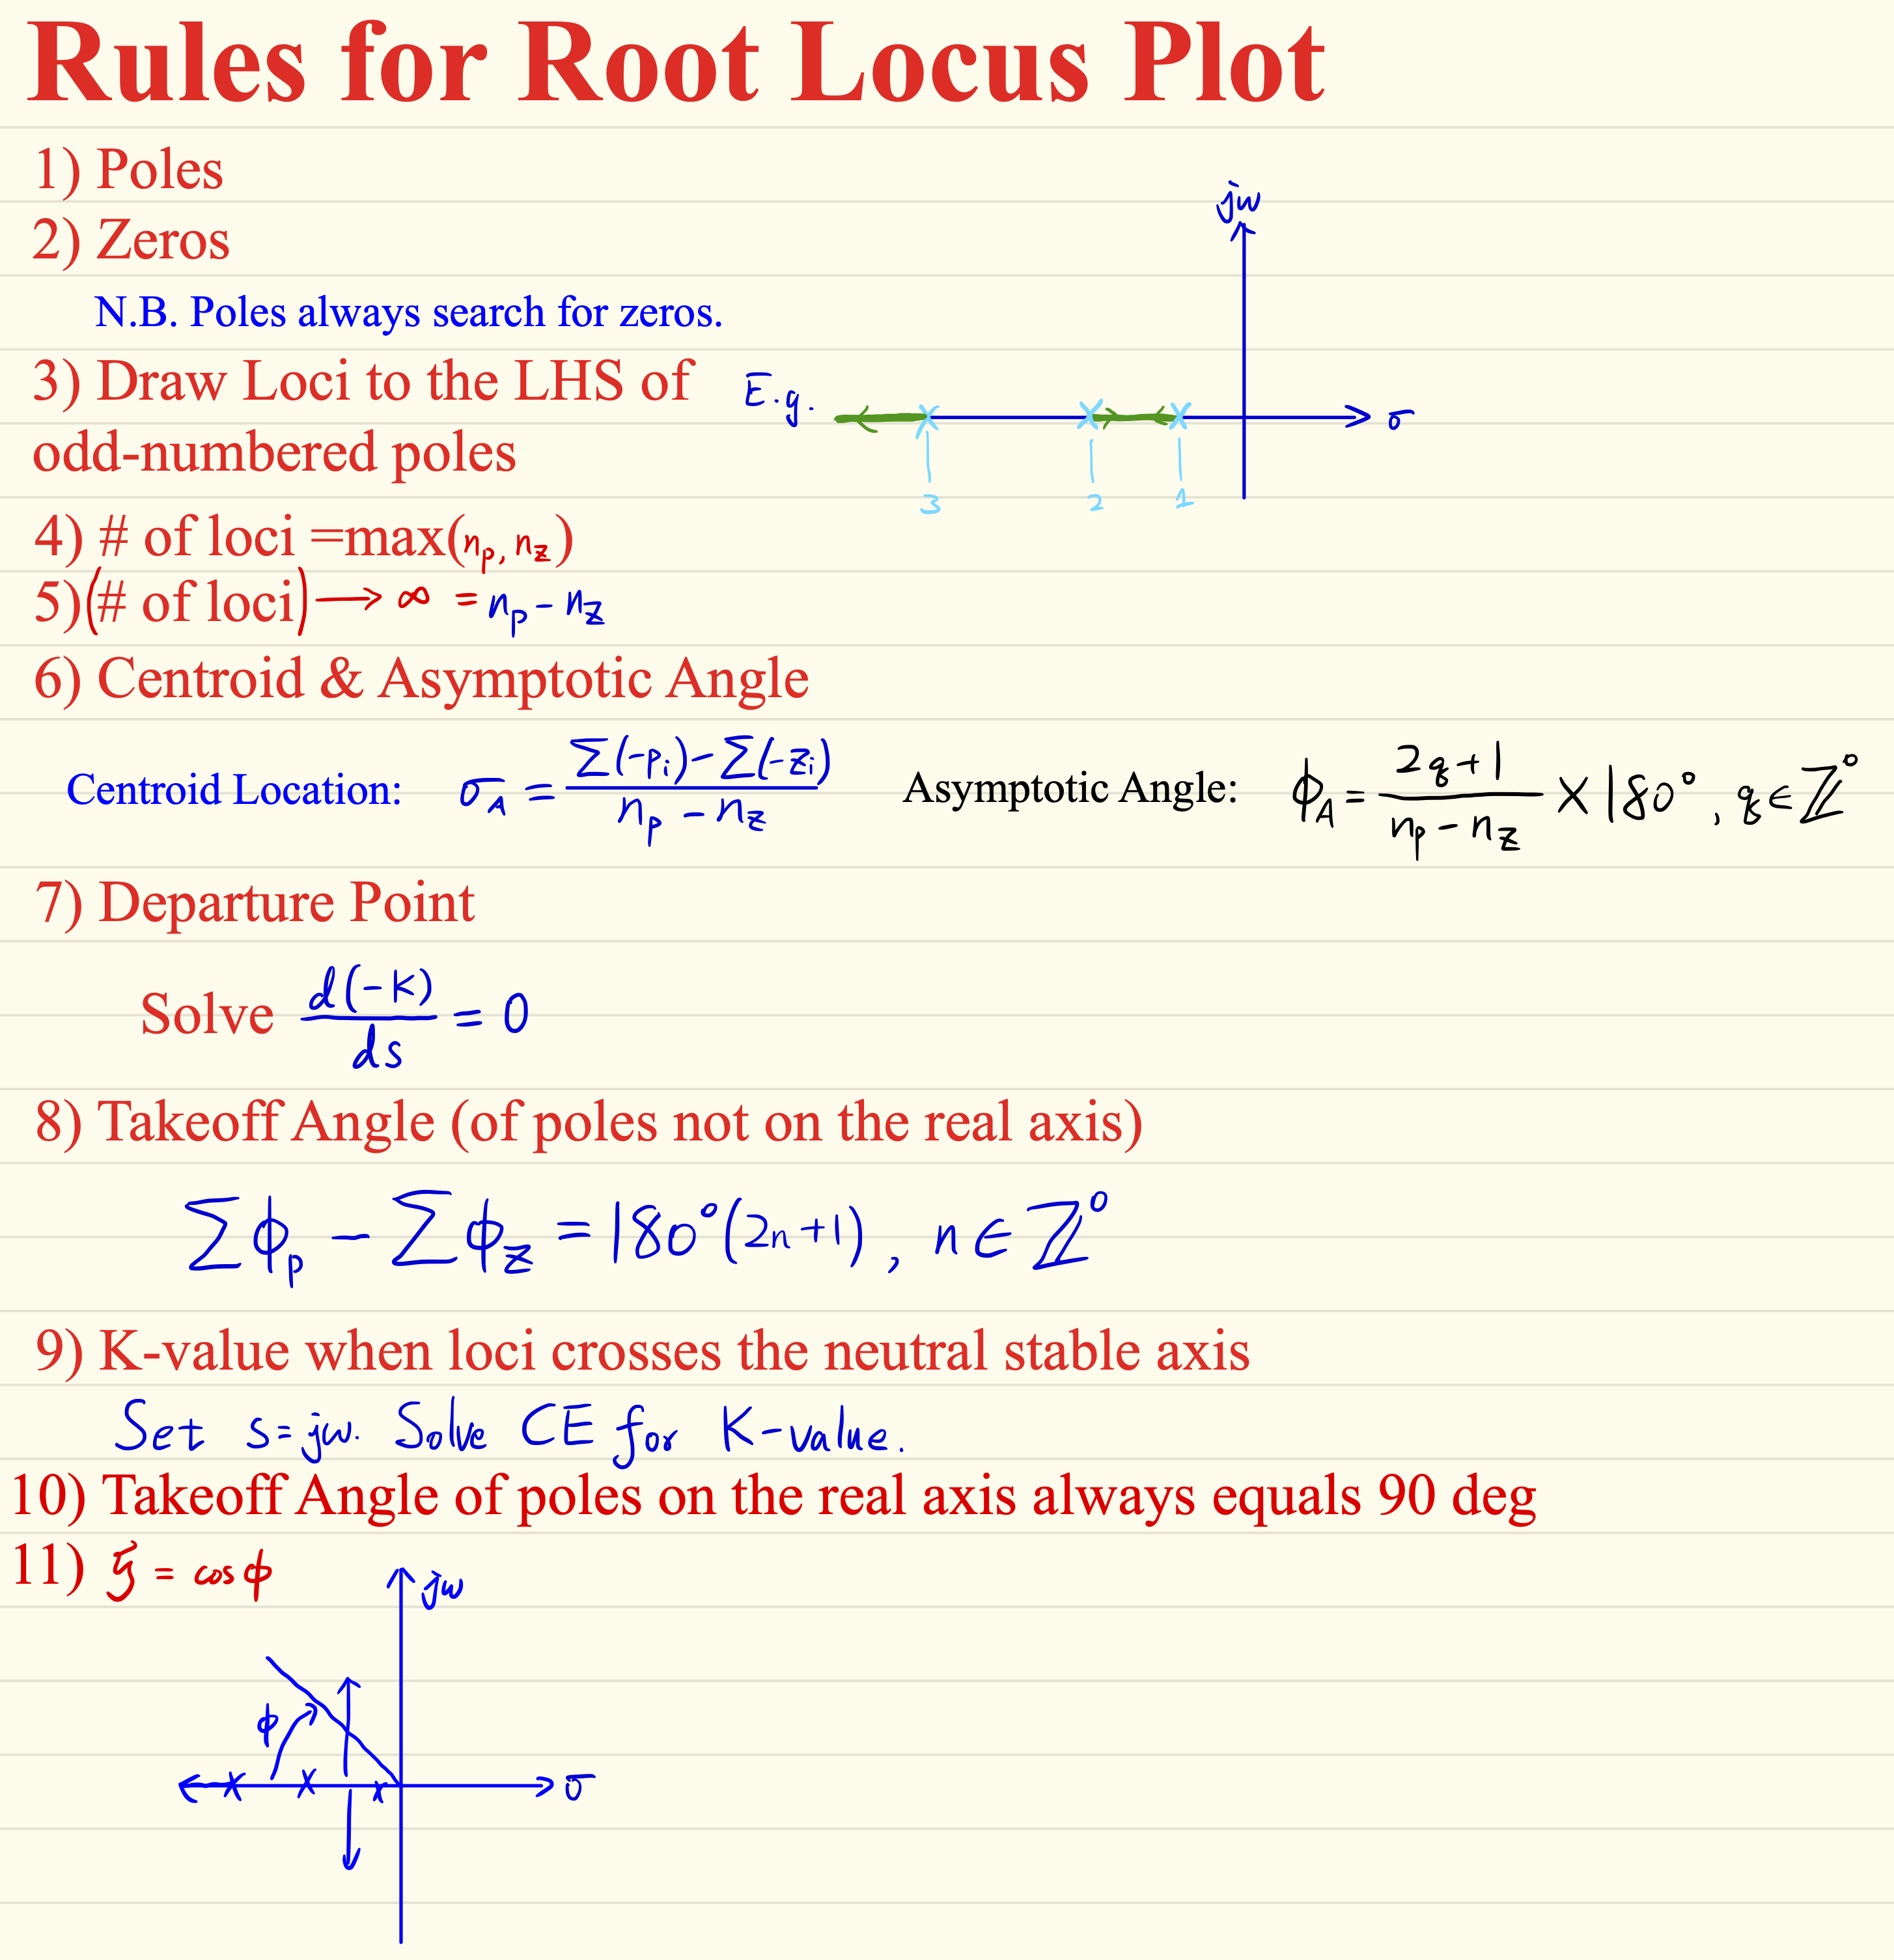
\includegraphics[width=0.5\textwidth]{images/root_locus_rules.png}
\end{figure}
\section{Week 4}
\textbf{\large $\bm{\mathcal{Z}}$-transform}
\begin{itemize}
    \item $\bm{\mathcal{Z}\Longleftrightarrow\mathcal{S}}$
    \begin{equation*}
        z = e^{sT}
    \end{equation*}
    \item $\bm{\mathcal{Z}\Longleftrightarrow\;}$\textbf{discrete time} by hand (and tables)
    \begin{align*}
        y(k+2) + y(k+1) + y(k) - y(k-1) &= u(k) \\
        \xrightarrow{\mathcal{Z}} z^2 Y(z) + zY(z) + Y(z) - z^{-1} Y(z) &= U(z)
    \end{align*}
    \item $\bm{\mathcal{Z}\Longleftrightarrow\;}$\textbf{discrete time} by almighty \textbf{Wolfram Alpha}: 
    
    Type \textit{"inverse Z transform calculator"} 
    
    or \textit{"Z transform calculator"} in the search bar.
\end{itemize}






\textbf{\large Transfer function of ZOH}
\begin{equation*}
    G_{ZOH}(s) = \frac{1-e^{-sT}}{s} 
\end{equation*}

\textbf{\large TF of ZOH + Analogy System (ZAS)}
\begin{align*}
    G_{ZAS}(z) &= \mathcal{Z}\left\{\frac{1-e^{-sT}}{s}G_{p}(s)\right\} \\
    &=  (1-z^{-1})\mathcal{Z}\left\{\frac{G_p (s)}{s}\right\} \\
    &= \frac{z-1}{z} \mathcal{Z}\left\{\frac{G_p (s)}{s}\right\}
\end{align*}

\textbf{\large Trick for finding inverse $\mathcal{Z}$-transform}

Divide the expression by z first, then find inverse using tables.

Example:
\begin{align*}
    Y(z) &= \frac{z^2}{(z-1)(z-0.5) } \\
    \frac{Y(z)}{z} &= \frac{z}{(z-1)(z-0.5)} = \frac{2}{z-1} - \frac{1}{z-0.5} \\
    Y(z) &= \frac{2z}{z-1} - \frac{z}{z-0.5} \\
    y(k) &= \mathcal{Z}^{-1}\left\{\frac{2z}{z-1}\right\} - \mathcal{Z}^{-1}\left\{ \frac{z}{z-0.5}\right\} \\
    &= 2 - 0.5^{k}
\end{align*}

\textbf{\large Associativity of Continuous Transfer Functions}
\begin{figure}[H]
    \centering
    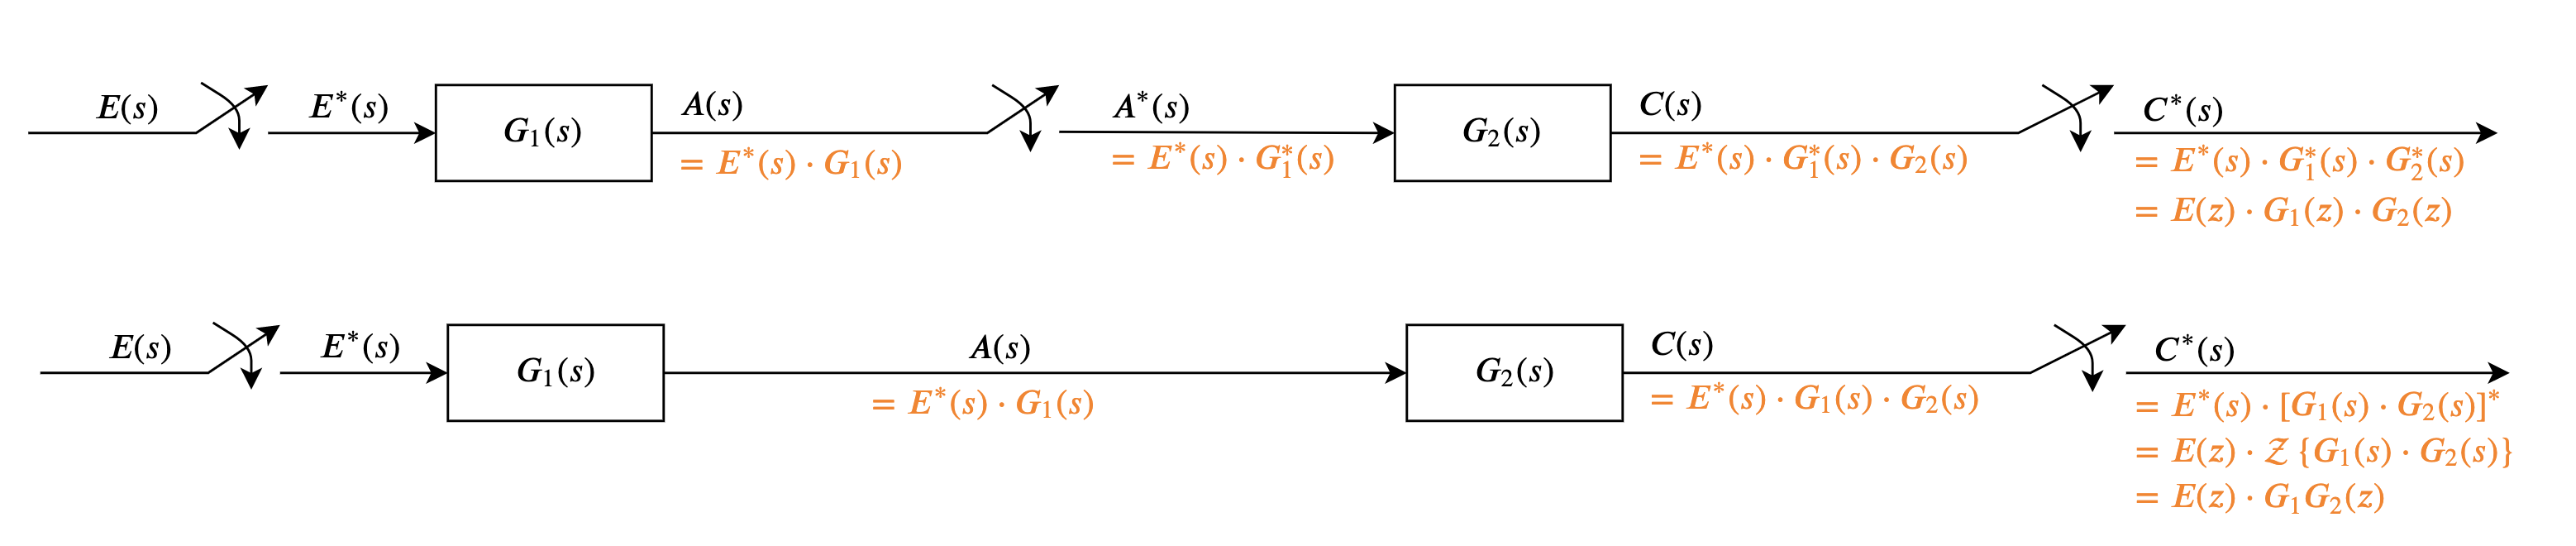
\includegraphics[width=0.5\textwidth]{images/associativity.png}
\end{figure}
Be careful: only distribute the * sign among addition/subtraction!


\section{Week 5}
\textbf{\large $\mathcal{Z}$-plane stability:}
\vspace{0.4cm}


\textbf{\underline{Case 1: z is real}}
\begin{figure}[H]
    \centering
    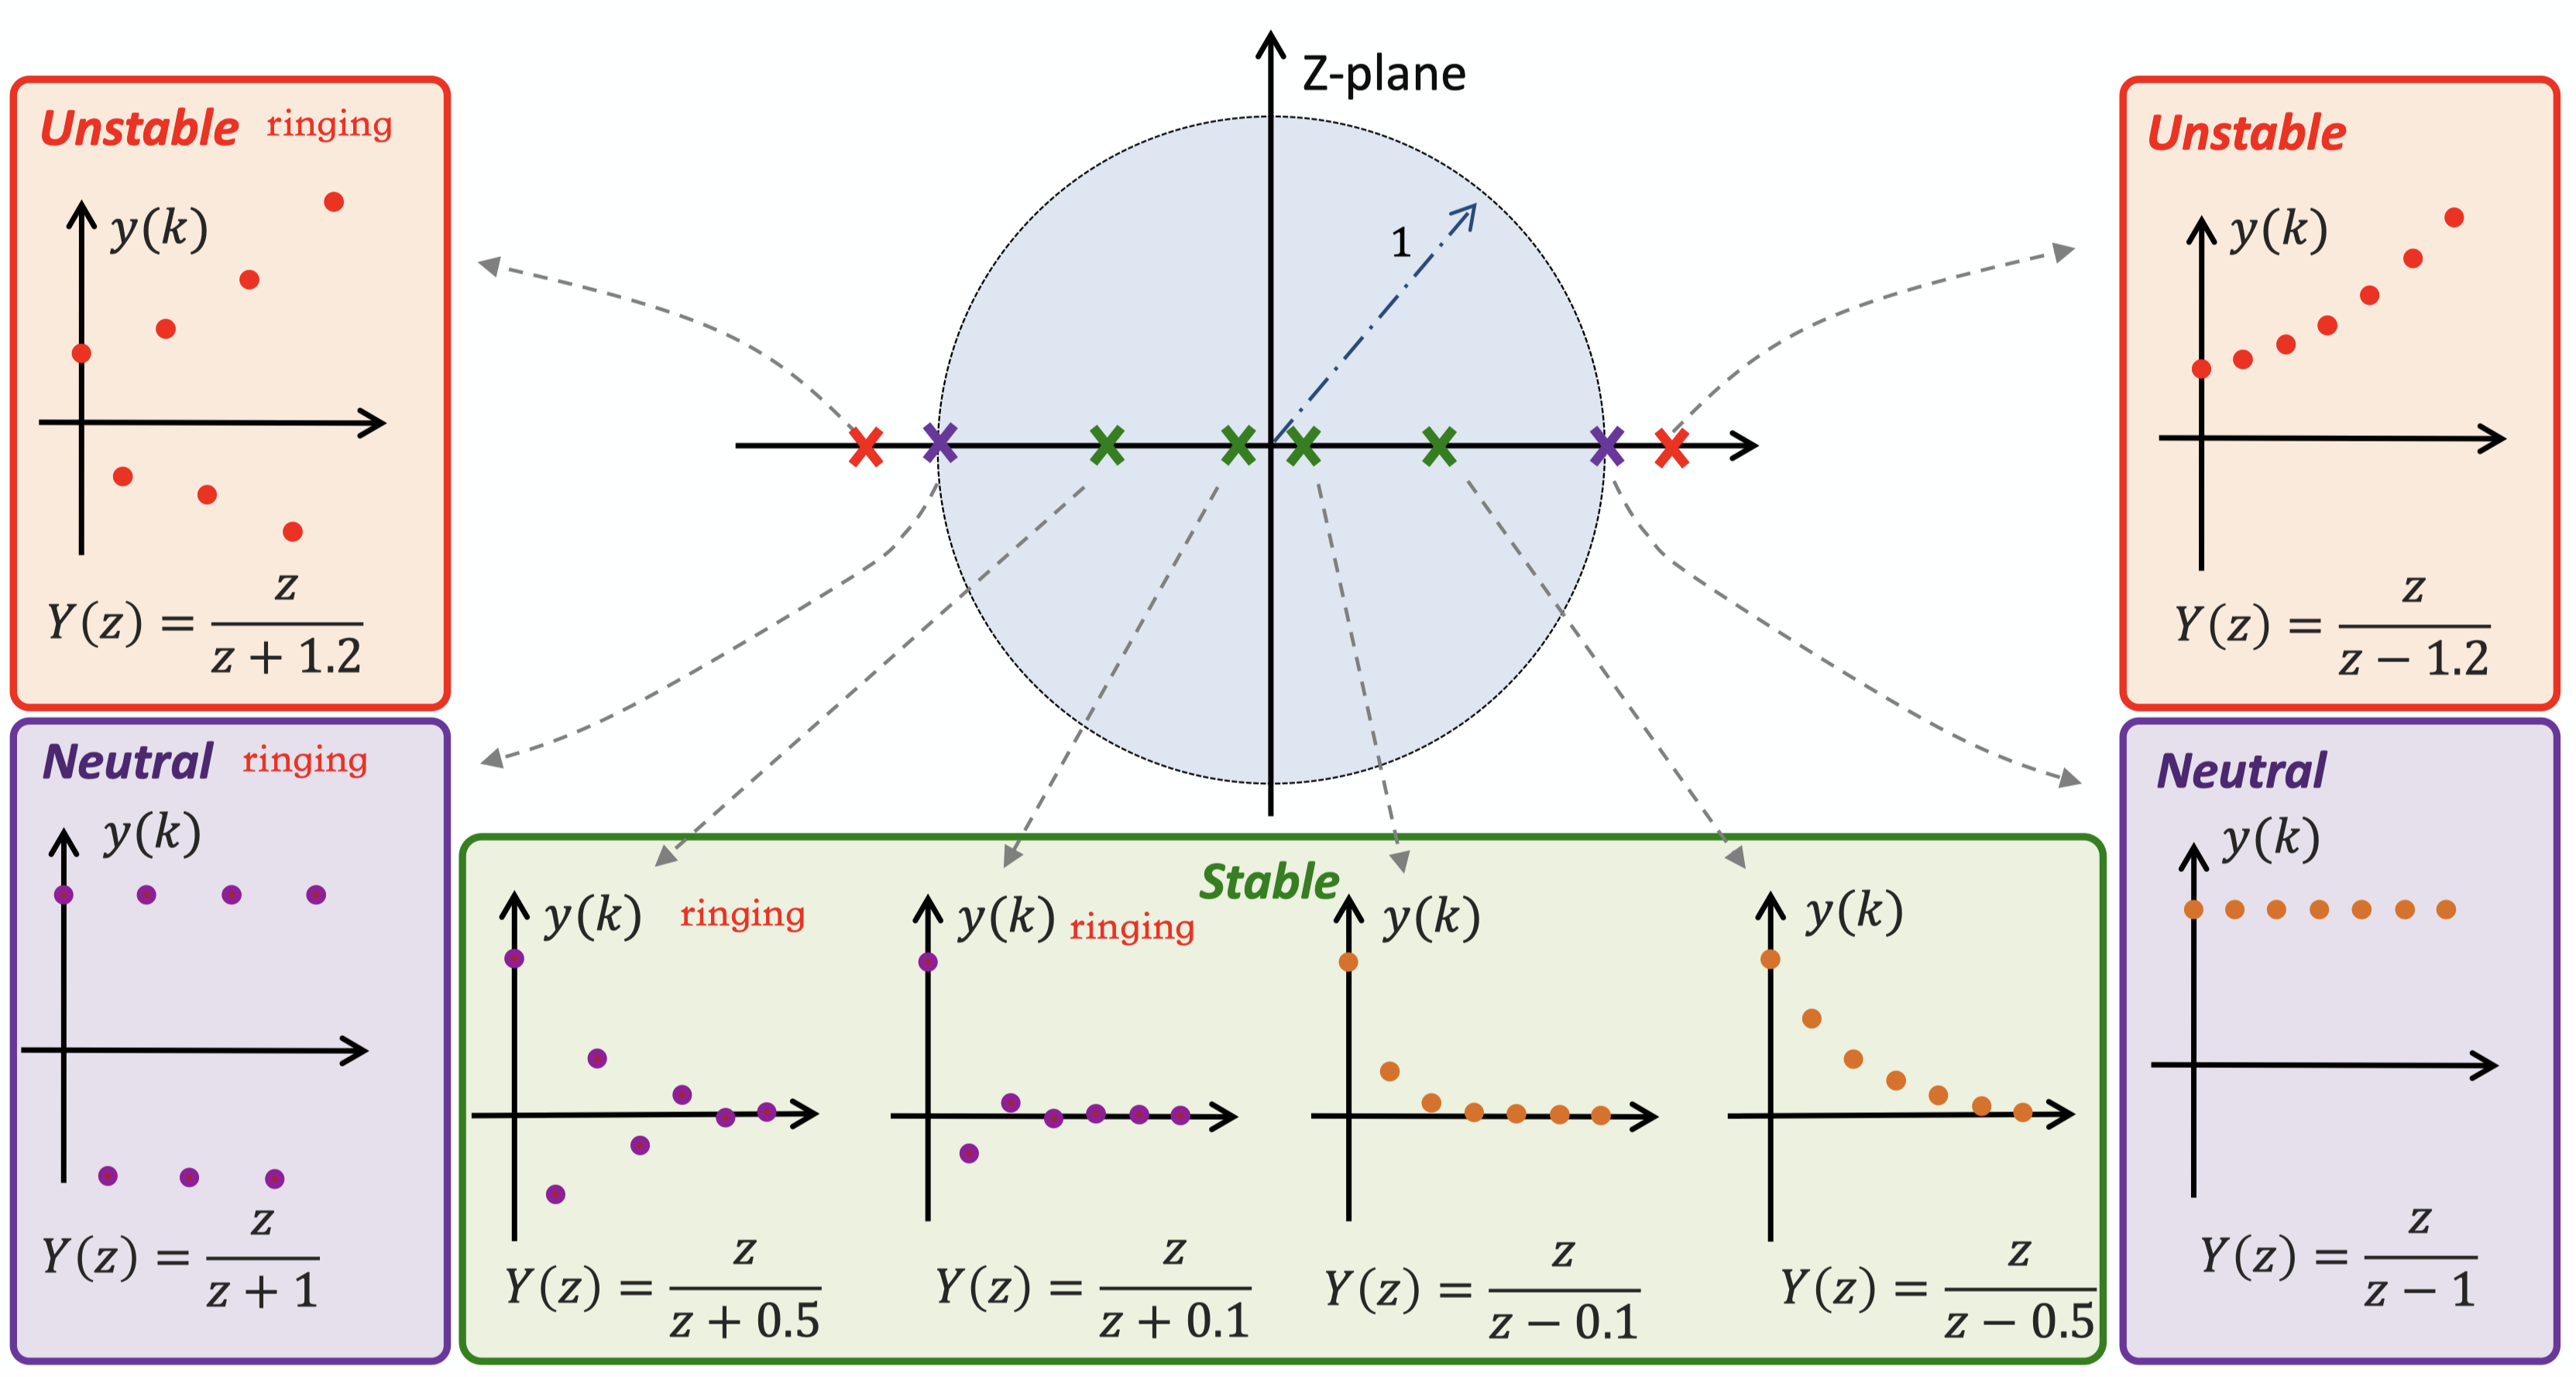
\includegraphics[width=0.5\textwidth]{images/z_plane_stability.png}
\end{figure}

\begin{table}[h]
\begin{adjustbox}{max width=\textwidth}
\begin{tabular}{|c|p{0.2\textwidth}|c|c|}
\hline
\textbf{$z=a$} & \textbf{transient response} & \textbf{stability} & \textbf{ringing?} \\\hline
$a> 1$ & transient term will grow & unstable & No \\\hline
$a = 1$ & transient term will remain constant & neutral & No \\\hline
$0<a<1$ & transient term will die down & stable & No \\\hline
$a=0$ & transient term will disappear in one sampling interval & stable & No \\\hline
$-1<a<0$ & transient term will disappear & stable & Yes \\\hline
$a = -1$ & transient term will ring with constant amplitude & neutral & Yes \\\hline
$a < -1$ & transient term will ring and grow & unstable & Yes \\\hline
\end{tabular}
\end{adjustbox}
\end{table}

\textbf{\underline{Case 2: z is complex}}
\begin{table}[h]
\begin{adjustbox}{max width=\textwidth}
\begin{tabular}{|c|c|c|}
\hline
\textbf{$z=p\pm jq = re^{\pm j\theta}$} & \textbf{$Cr^k \cos(k\theta + \phi)$} & \textbf{stability} \\\hline
$r\ge 1$ & oscillatory, grow to $\infty$ & unstable \\\hline
$r=1$ & oscillatory, stay steady & neutral $a=-1$ \\\hline
$0<r<1$ & oscillatory, disappear as $t\to\infty$ & stable  \\\hline
$r=0$ & disappear in one sample interval & stable \\\hline
\end{tabular}
\end{adjustbox}
\end{table}

\textbf{\large Important Difference between s- and z-plane:} 
\begin{itemize}
    \item Double poles on the unit circle (a ramp) is not stable!
    \item System stable in s-domain for all value of $K$ is NOT necessarily stable in z-domain for all $K$ for certain sampling time $T$. Example: Kahoot wk7 Q9.
\end{itemize}

\textbf{\large $\mathcal{S}$-plane and $\mathcal{Z}$-plane Mapping}
\begin{equation*}
    s= e^{Ts} = e^{T(\sigma + j \omega)} = e^{T\omega} e^{T j\omega} = r e^{T j\omega}
\end{equation*}
N.B. not sure if $T$ should be included, since $T$ does not influence the plots in both s-domain and z-domain.
\begin{align*}
    s &= \sigma + j \omega_d \; \begin{cases}
    \sigma = \frac{\ln(r)}{T}\; , & |z| = r = e^{\sigma} \\
    \omega_d = \frac{\theta}{T} \; , & \angle z = \omega_d 
    \end{cases} \\
    C_0 &= -\frac{\sigma}{\omega} = - \frac{\ln(r)}{\theta} = -\sqrt{\frac{\zeta}{1-\zeta^2}} 
\end{align*}
\begin{figure}[H]
    \centering
    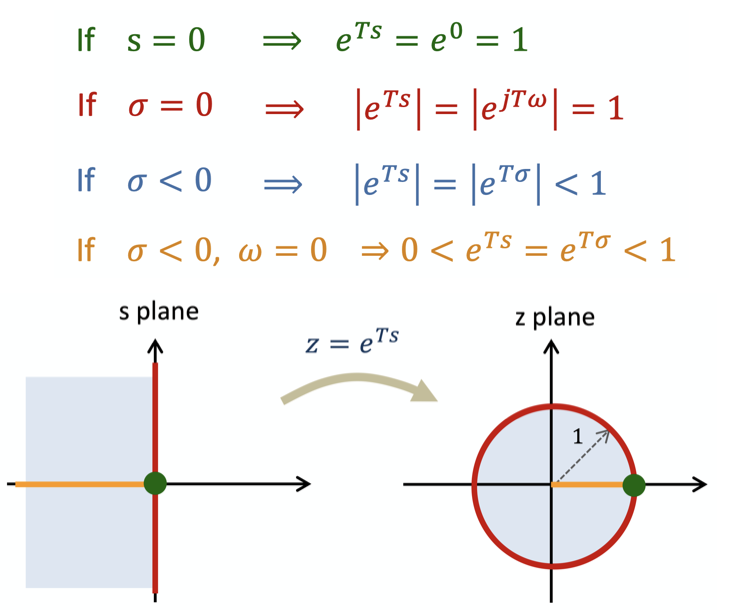
\includegraphics[width=0.5\textwidth]{images/s_z_mapping.png}
\end{figure}

\textbf{\underline{Critical Points:}}
\begin{itemize}
    \item Origin $s=0$ mapped to $z=e^0 = 1$ (real axis);
    \item Constant settling time / vertical line / $Re(s)=\sigma$ mapped to a circle $|z|=e^{\sigma}$ centered at origin:
    \begin{itemize}
        \item Line $Re(s)=-\infty$ mapped as the origin since $|z|=e^{-\infty}=0$;
        \item Im axis $Re(s)=0$ mapped as the unit circle since $|z|=e^0=1$;
        \item Line $Re(s)=\infty$ mapped as the circle of infinite radius since $|z|=e^{\infty}=\infty$.
    \end{itemize}
    \item Constant frequency line / horizontal line / $Im(s)=j\omega_d$ mapped as a ray starting from the origin with angle $\angle \omega_d$ ;
    \item The range $\omega_d \in (-\infty, \infty)$ is mapped to a finite range $\omega_d \in [0, 2\pi]$.
\end{itemize}

\begin{figure}[H]
    \centering
    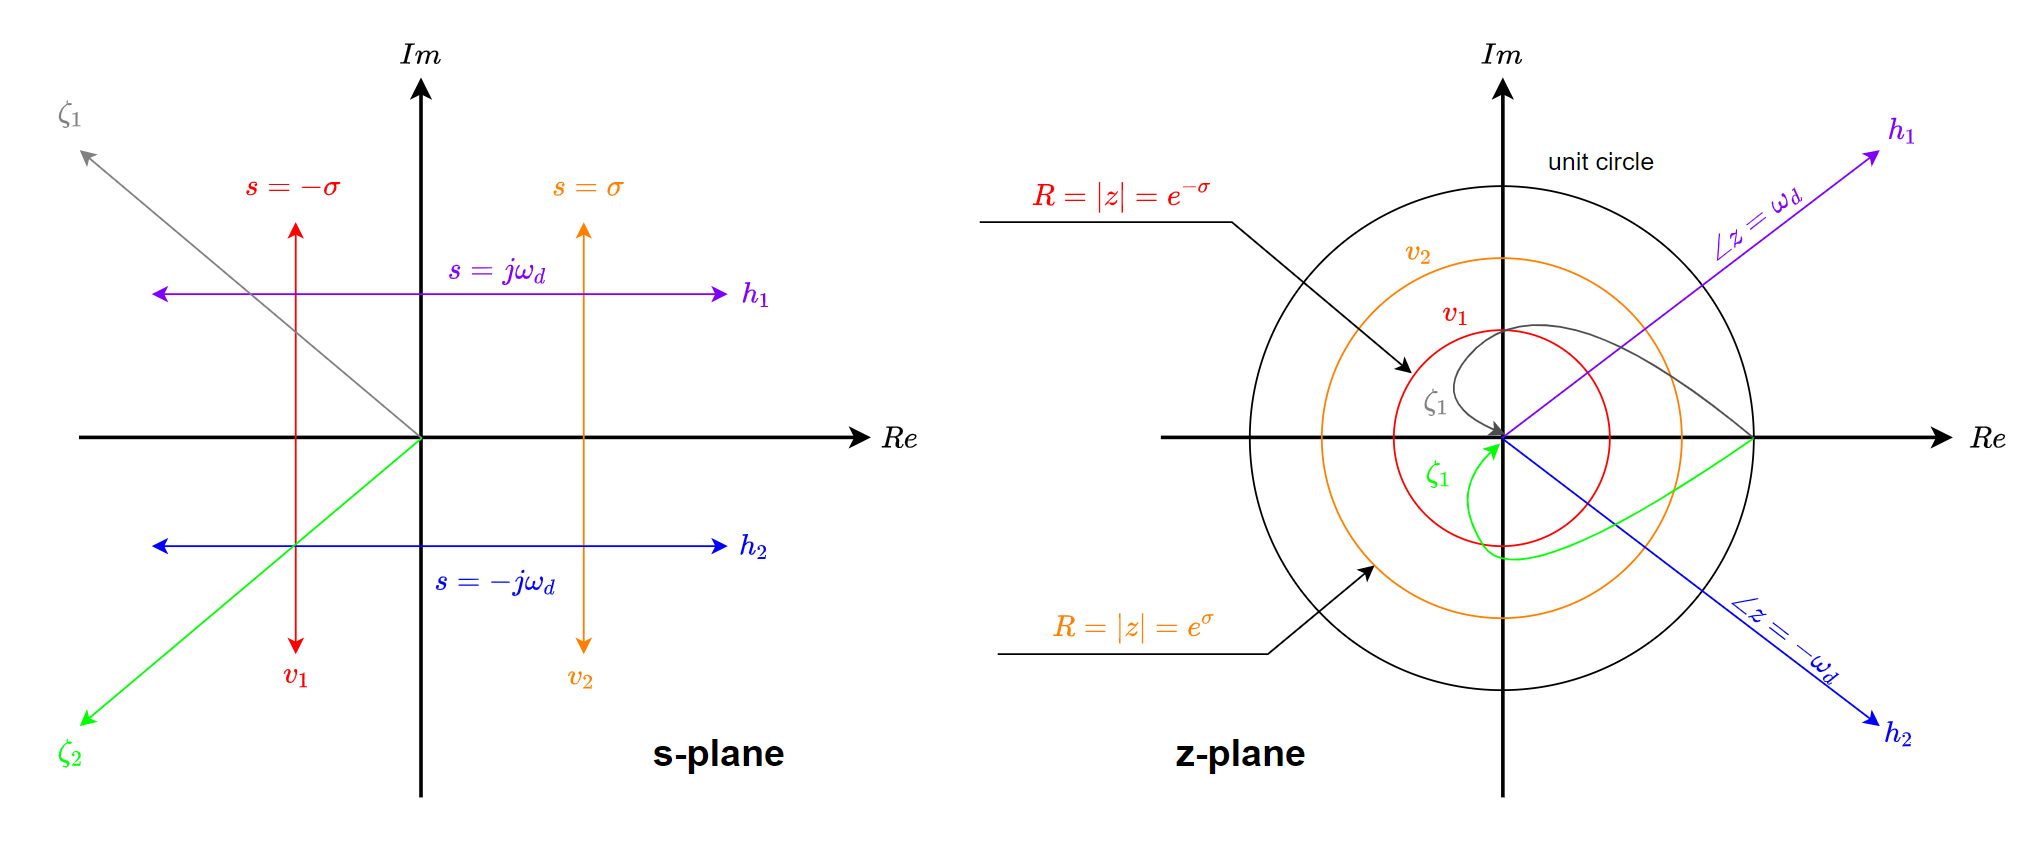
\includegraphics[width=1.0\linewidth]{images/Mapping_sumary_1.png}
\end{figure}
\begin{figure}[H]
    \centering
    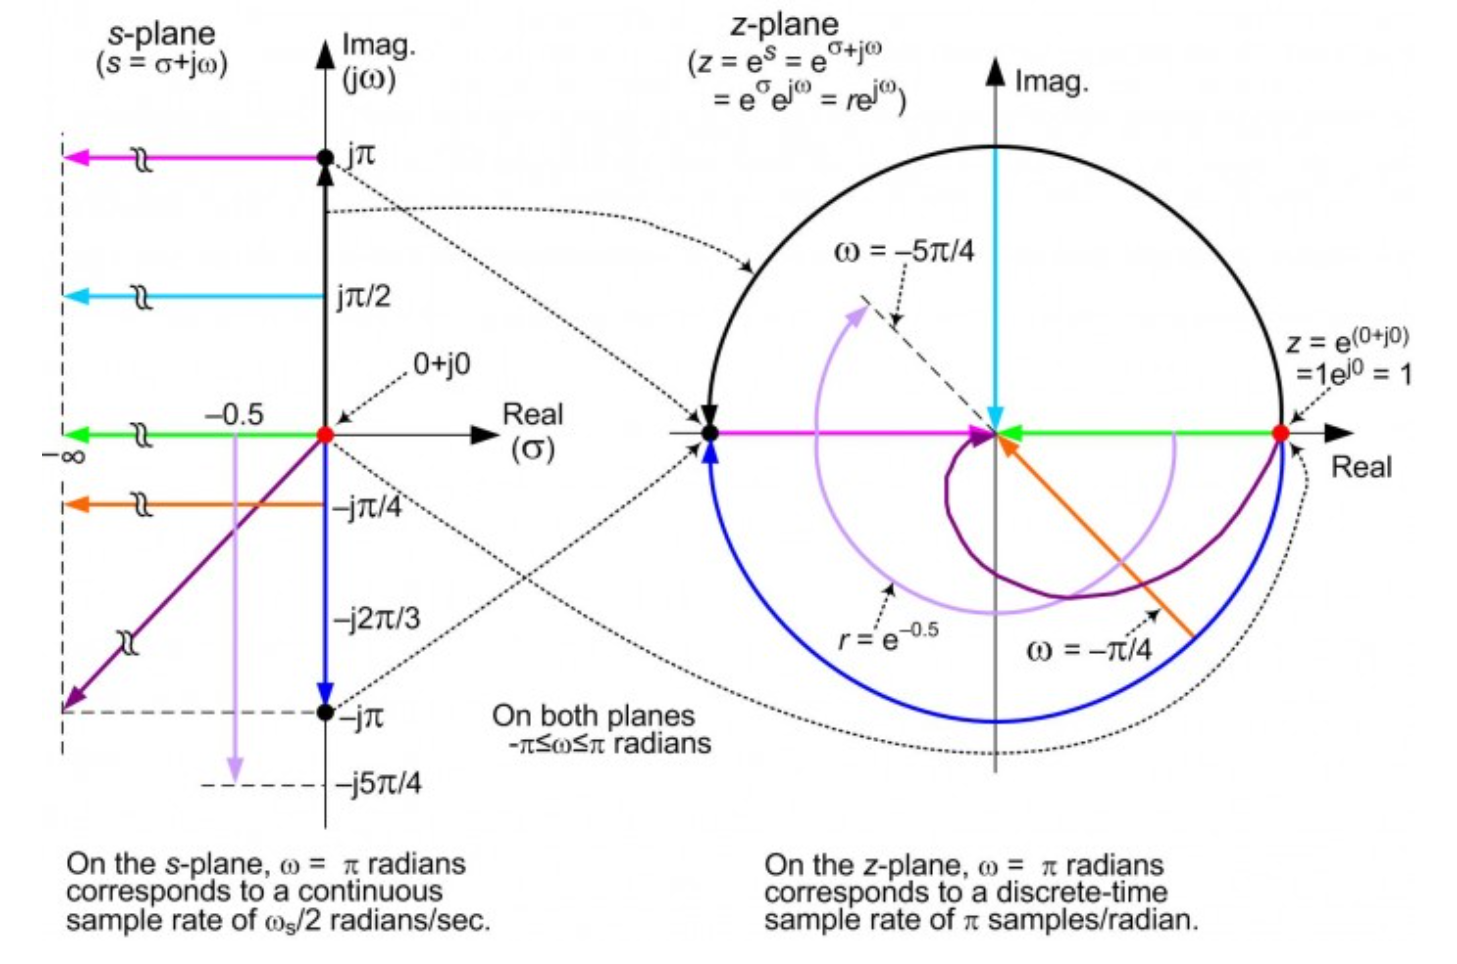
\includegraphics[width=1.0\linewidth]{images/Mapping_sumary_2.png}
\end{figure}

\textbf{\large Dominant poles in z-plane}: 
\begin{itemize}
    \item The poles closer to the unit circle are the dominant/slowest poles.
\end{itemize}


\textbf{\large Steady state gains}
\begin{itemize}
    \item \textbf{DC Gain} = $\lim_{z\to 1} G(z)$ 
    \item \textbf{Inst. Gain} = $\lim_{z\to \infty} G(z)$
\end{itemize}

\textbf{\large Discrete State Space}
\begin{equation*}
    \begin{cases}
     \dot{x}(t) = \bm{A}x(t) + \bm{B}u(t) \\
     y(t) = \bm{C}x(t)+\bm{D} u(t)
    \end{cases}, \; \begin{cases}
     x(k+1) = \bm{G}x(k) + \bm{H}u(k) \\
     y(kT) = \bm{C}x(kT) + \bm{D}u(kT)
    \end{cases}
\end{equation*}
\begin{align*}
    \text{where } \bm{G} &= e^{\bm{A}T} \\
    \bm{H} &= \int_{0}^{T}\left(e^{\bm{A}\lambda} d\lambda\right) \bm{B} \\
    &= \bm{A}^{-1} (e^{\bm{A}T}- \bm{I})\bm{B}
\end{align*}

\textbf{From z-pole to $\bm{\omega_d}$:}

\begin{enumerate}
    \item Given that $z=a+j\, b$, $T$ is known,
    \item From $z=e^{sT}$ we have $s=\frac{\ln(a+j\, b)}{T}=\sigma + j\, \omega_d$
\end{enumerate}

\textbf{From z-pole to 95\% $\bm{t_s}$:}
\begin{enumerate}
    \item $s = \frac{\ln(z)}{T} = \sigma + j\,\omega_d$ ,
    \item $e^{\sigma \, t_s} = 1 - 0.95$,
    \item $t_s = \frac{\ln(1-0.95)}{\sigma}\;$, ($t_s$ should be +ve).
\end{enumerate}
\section{Week 7}
\textbf{\underline{Pole-Zero Placement}}

When a transfer function is given,
\begin{equation*}
    G_p (z) = \frac{z-0.1}{(z-0.8)\cdot (z^2-z+0.34)} \; ,
\end{equation*}

and the question asks for a pole/zero placement that makes the system goes through a certain point that was not originally on the root locus,
\begin{equation*}
    z^* = 0.4+j\,0.17 \; ,
\end{equation*}

Do the following steps:
\begin{enumerate}
    \item Compute $G_p(z^*)$. In this example,
    \begin{align*}
        G_p(z^*) &= -1.38451 - j\, 9.3625 \\
        &= 9.46432 \, \angle -98.41^{\circ} 
    \end{align*}
    \item Obtain the angle contribution the controller needs to provide. In this case,
    \begin{align*}
        \theta &= -180^{\circ} - (-98.41^{\circ}) \\
        &= -81.58^{\circ} 
    \end{align*}
    \item Use geometry to determine the pole/zero location (not sure if there's a better and quicker way).
\end{enumerate}
\begin{figure}[h]
    \centering
    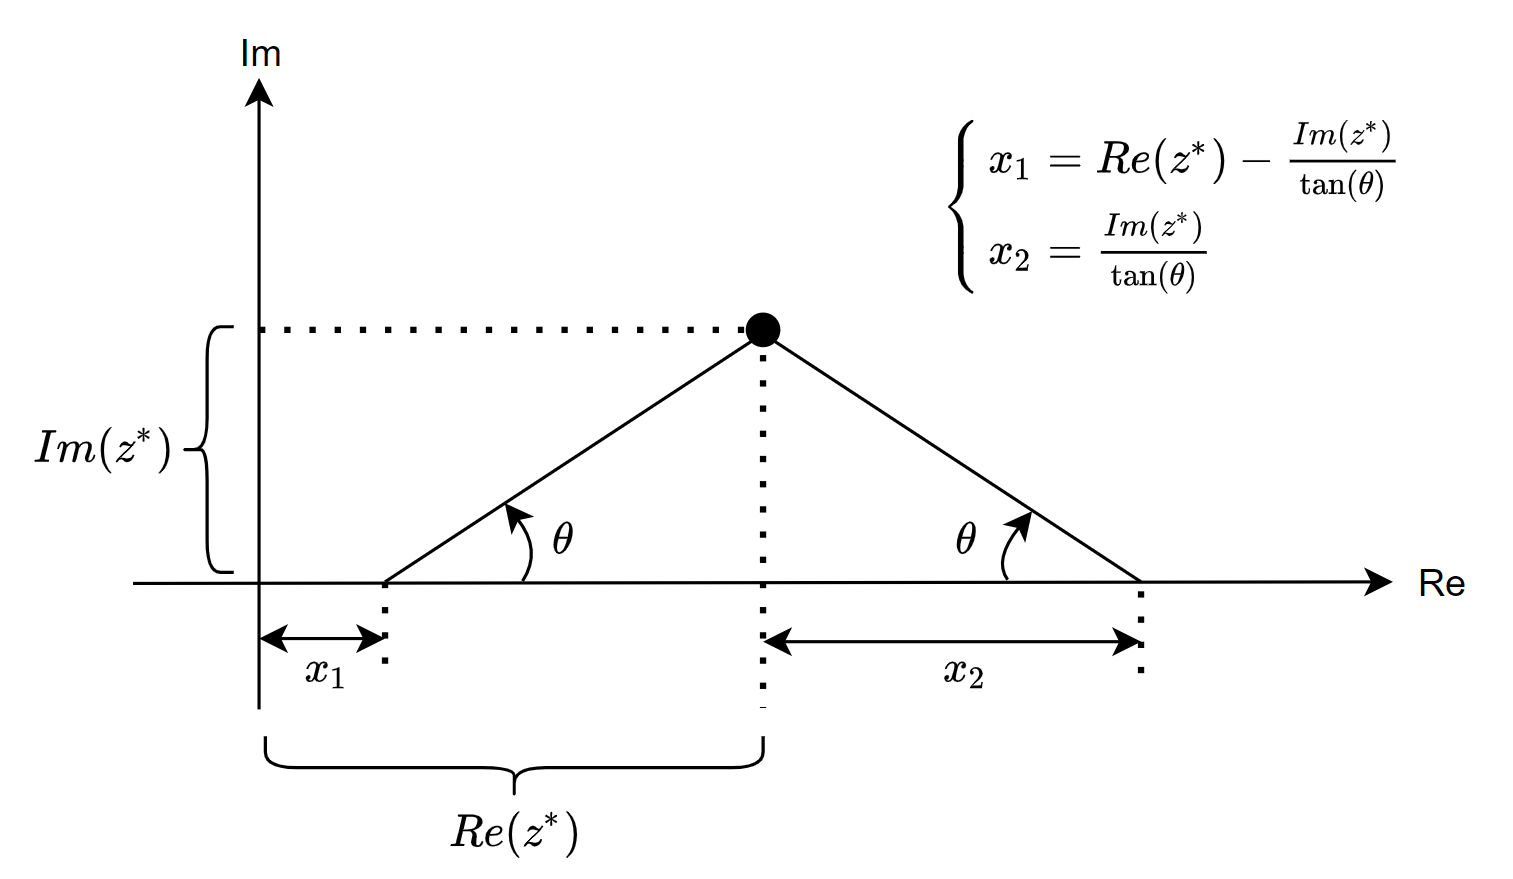
\includegraphics[width=1.0\linewidth]{images/pole_placement.png}
\end{figure}
    
\textbf{\large Cancellations:}
\begin{itemize}
    \item Cancellation of unstable poles of $G_p$ at the implementation stage leads to instability, because the value of physical poles cannot be precisely measured.
    \item Cancellation taken place at the computational plane is harmless.
    \item Cancel a pole with real parts greater than 0 in z-domain is more worrisome than cancelling a pole with negative real part.
    \begin{equation*}
        \begin{cases}
            \frac{4(z+0.5)}{(z+0.5)(z-0.1)} \\
            y(k) = C_1 (-0.5)^k + C_2 (0.1)^k
        \end{cases}
    \end{equation*}
    Ex. $(z-0.1)$ is the more worrying pole because $C_2 (0.1)^k$ is growing while $C_1 (-0.5)^k$ is neutral and ringing.
\end{itemize}

\clearpage
\section{Useful MATLAB Functions}

\underline{\textbf{Set up Transfer Function}}

Given transfer function in s-domain
    \begin{equation*}
        G = \frac{s-3}{(s+1)(s+2)} = \frac{s-3}{s^2+3s+2}
    \end{equation*}

\begin{lstlisting}
% Approach 1
s = tf('s');
Gs = (s-3) / ( (s+1) * (s+2) );
% Approach 2
num = [1 -3];
den = [1 3 2];
Gs = tf(num,den);
% Approach 3
num = [1 03];
den = conv([1 1],[1 2]);
Gs = tf(num,den);
%% If in z-domain ...
T = -1;
z = tf('z', T);  % T=-1 means sampling time
                 % unspecified
% rest are similar
\end{lstlisting}

Given pole locations as
\begin{equation*}
    z_{1,2} = 1.87 \pm j\, 1.36
\end{equation*}

\begin{lstlisting}
z1 = 1.87 + 1i * 1.36; 
z2 = 1.87 - 1i * 1.36;
den = poly([z1,z2])
>> den = 1.0000   -3.7400    5.3465
\end{lstlisting}

Given plant transfer function in s-domain and sampling time, find ZAS:
\begin{equation*}
    \text{Given } \begin{cases}
    G_p(s) = \frac{1}{s(s+1)} \\
    T = 0.04 \; \text{sec}
    \end{cases}
\end{equation*}
\begin{lstlisting}
num_c = [1];
den_c = [1 1 0];
T = 0.04;  % cannot set to -1 for 
           % unspecified case
[num_d den_d] = c2dm(num_c,den_c,T,'zoh');
Gp_zas = tf(num_d,den_d,T)
\end{lstlisting}

Given CE as follow, find roots.
\begin{equation*}
    \text{CE} = \frac{9/8}{z^2+1.5z+9/8}
\end{equation*}
\begin{lstlisting}
CE = tf([9/8], [1 1.5 9/8], -1); % T=-1
zeors = roots(cell2mat(CE.Num));
poles = roots(cell2mat(CE.Den))
>> poles =
  -0.7500 + 0.7500i
  -0.7500 - 0.7500i
\end{lstlisting}



\textbf{\underline{Other Minutiae:}}
\begin{itemize}
    \item Instantaneous Gain: \textbf{Wolfram Alpha}.
    \item DC Gain:
\end{itemize}
\begin{lstlisting}
% Case 1: in s-domain
dcgain(sys_s);
% Case 2: in z-domain
evalfr(sys_z, 1) % since G(1) = DC. G.
\end{lstlisting}

\begin{itemize}
    \item Partial fraction decomposition:
    \begin{align*}
        \text{Given that }\; \frac{-4s+8}{s^2+6s+8} \\
        \text{want: }\, \frac{-12}{s-(-4)} + \frac{8}{s-(-2)}
    \end{align*}
\end{itemize}
\begin{lstlisting}
num = [-4 8];
den = [1 6 8];
[r p k] = residue(num,den)
>> r = [-12 
          8]
>> p = [-4 
        -2]
>> k = []        
\end{lstlisting}


\textbf{\underline{Transformation Summary}}
\begin{figure}[h]
    \centering
    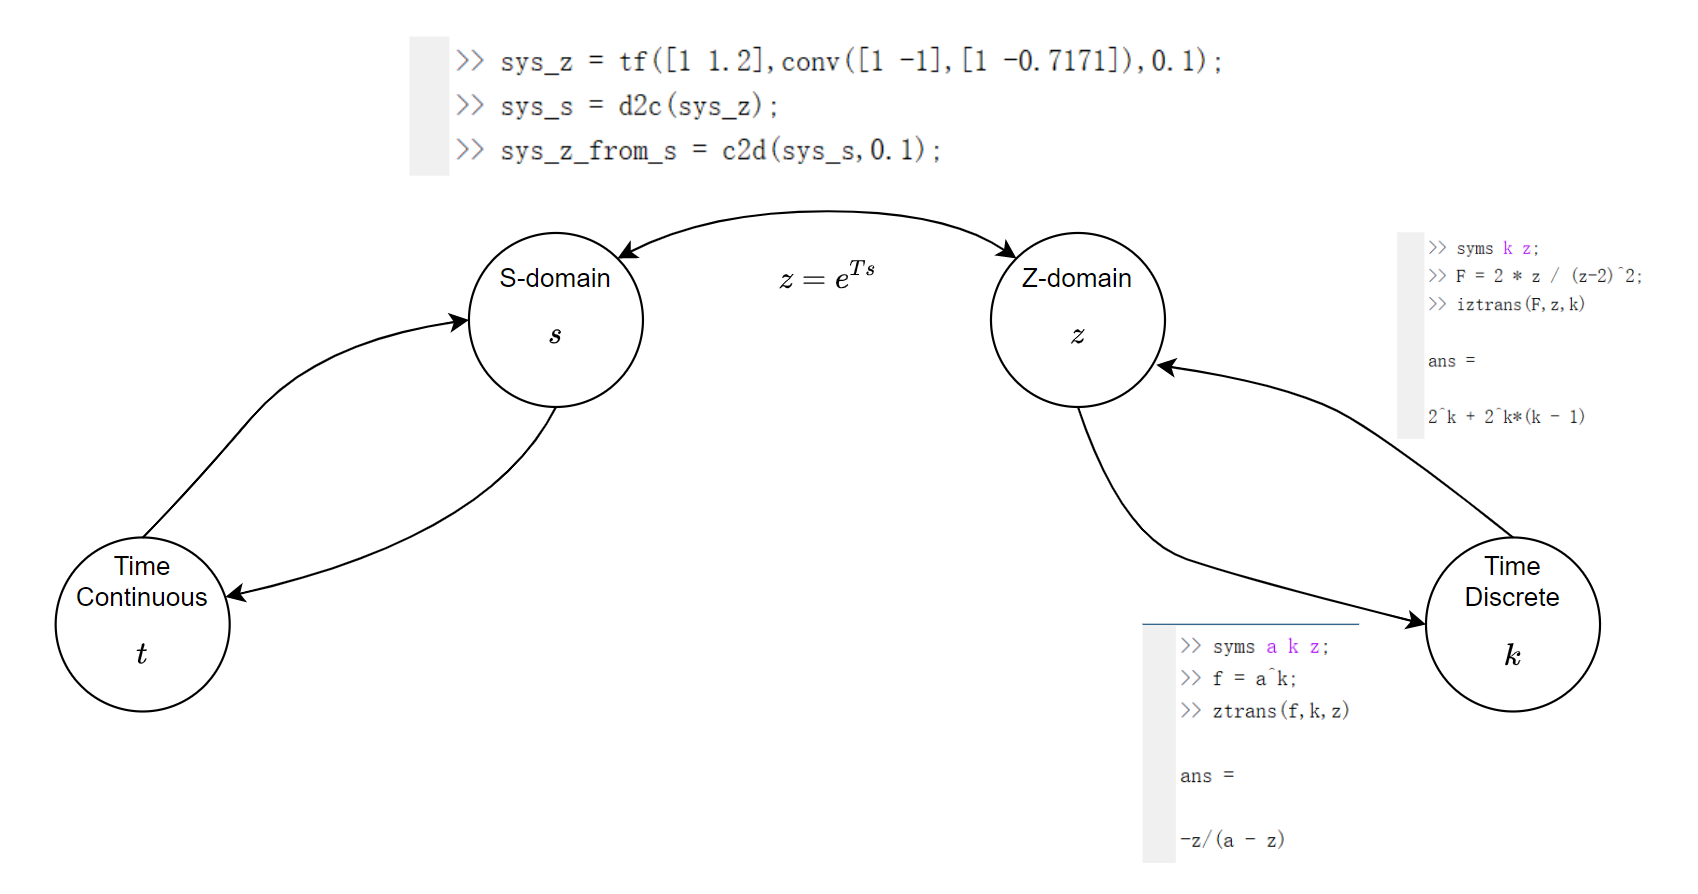
\includegraphics[width=1.0\linewidth]{images/transformation_Summary.png}
\end{figure}

\printbibliography


\end{document}